% !TEX root = ../stellar-notes.tex
Stars form in clouds of mostly molecular hydrogen embedded in the interstellar medium (ISM).
These molecular clouds have typical temperatures of 10--20 K and number densities of $10^3$--$10^4$ g cm$^{-3}$.
This is far denser than typical phases of the ISM ($\lesssim50$ g cm$^{-3}$).
Turbulence in these clouds results in density perturbations which can become gravitationally unstable and collapse to ultimately form stars.

In this chapter, we will present the basics behind star formation, from the conditions for collapse of cold molecular cores to the formation of radiative pre-main sequence stars.

\section{The Jeans' criterion}

Local overdensities in turbulent molecular clouds in the ISM must reach a minimum size in order to become gravitationally unstable.
We can derive this minimum core size by reviewing a classic piece of stability analysis.
Let's consider the collapse of a homogeneous, isotropic fluid. Our equations are conservation of mass and momentum, plus Poisson's equation for the gravitational potential:
\begin{eqnarray}
\partial_{t}\rho + \divr(\rho \vu) &=& 0\label{e.jeans-mass-cons}\\
\partial_{t}(\rho\vu) + \divr(\rho\vu\vu) &=& - \rho \grad\Phi - \grad P\label{e.jeans-momentum}\\
\nabla^{2} \Phi &=& 4\pi G \rho\label{e.jeans-poisson}.
\end{eqnarray}
Right away we run into a snag: if our system is homogenous and isotropic, then $\grad\Phi = 0$, since there is no preferred direction for the vector to point. In this case the left-hand side of Poisson's equation vanishes, which is inconsistent with our having a background density.  This, of course, is the central point to cosmology, and if we want to do this calculation correctly we need general relativity and an expanding background universe.

Instead, we shall take an alternate route: following Jeans' lead, we simply assert that there is a background state of uniform density $\rho_{0}$. This is known as the Jeans Swindle \citep[c.f.,][]{binney:1987} and, while not quite consistent, still provides insight.
Forging ahead, we write the density, velocity, and potential as a background piece (subscript ``0'') plus a perturbation (subscript ``1''):
\begin{eqnarray*}
\rho(\vx,t) &=& \rho_{0} + \rho_{1}\exp(i\bvec{k}\vdot\vx - i\omega t)\\
\vu(\vx,t) &=& \vu_{1}\exp(i\bvec{k}\vdot\vx - i\omega t)\\
\Phi(\vx,t) &=& \Phi_{1}\exp(i\bvec{k}\vdot\vx - i\omega t).
\end{eqnarray*}
Here, $k$ is the wavenumber of the perturbations and has the usual relation to wavelength, $k = 2\pi/\lambda$.
We take the perturbations to be adiabatic: $\dif P = c_{s}^{2}\dif\rho$.

Re-writing Eq. (\ref{e.jeans-mass-cons}) in perturbed form gives,
\newcommand{\expikx}{\ensuremath{e^{i\bvec{k}\cdot\bvec{x}-i\omega t}}}
\newcommand{\expikxb}{\ensuremath{e^{i{k}{x}-i\omega t}}}
\[ \partial_t (\rho_1 \expikx) + \nabla\cdot(\rho_0\bvec{u}_1\expikx + \rho_1\bvec{u}_1 \expikx)x.  \]
We shall drop all terms higher than first order in the perturbation and so the second term in the divergence is zero.
Furthermore, we shall pick a direction by dotting $\bvec{k}$ into the perturbed equations, yielding
\[
  -i\omega \rho_1 \expikxb + i k \rho_0 u_1 \expikxb = 0,
\]
or
\begin{equation}
  u_1 = \frac{\omega \rho_1}{k \rho_0}. \label{e.jeans1}
\end{equation}
Similarly, for Poisson's equation (\ref{e.jeans-poisson}) we have
\[ \nabla^2 (\Phi_1 \expikx) = 4\pi G \rho_1\expikx, \]
where we remember the Swindle and drop the dependence on $\rho_0$.
Dotting by \bvec{k} and taking a couple spatial derivatives gives
\[ -k^2 \Phi_1 \expikxb = 4\pi G \rho_1 \expikxb,  \]
or
\begin{equation}
  \Phi_1 = -\frac{4\pi G}{k^2} \rho_1. \label{e.jeans2}
\end{equation}
Finally, for the momentum equation (\ref{e.jeans-momentum})
\begin{eqnarray*}
  \partial_t (\rho_0 \bvec{u}_1\expikx + \rho_1\expikx\bvec{u}_1\expikx) = \\
  -\grad(c_s^2\rho_0 + c_s^2\rho_1\expikx) - (\rho_0+\rho_1\expikx)\grad(\Phi_1\expikx),
\end{eqnarray*}
where we have already dropped all terms in the divergence since they are all second order or higher and we have used the adiabatic relation for $P$.
Dotting by $\bvec{k}$ and taking some derivatives, we have
\begin{eqnarray*}
 -i\omega\rho_0 u_1 \expikxb &=& -i k c_s^2\rho_1\expikxb - i\rho_0 k \Phi_1\expikxb \\
 \omega\rho_0 u_1 &=& k c_s^2\rho_1 + \rho_0 k \Phi_1.
\end{eqnarray*}
Using Eqs. (\ref{e.jeans1}) and (\ref{e.jeans2}) to eliminate $u_1$ and $\Phi_1$ gives us
\begin{eqnarray}
  \omega^2\rho_1 &=& k^2 c_s^2\rho_1 - 4\pi G\rho_0 \rho_1 \nonumber\\
  \omega^2 &=& k^2 c_s^2 - 4\pi G\rho_0. \label{e.jeans-dispersion}
\end{eqnarray}

Equation (\ref{e.jeans-dispersion}) is the {\it dispersion relation} for the Jeans instability.
For sufficiently small $k$ (long wavelengths) $\omega^{2}<0$ and the perturbations will grow exponentially. Setting $\omega = 0$ defines the \textbf{Jeans' length},
\begin{equation}\label{e.Jeans-length}
\lambda_{\mathrm{J}} = c_{s}\sqrt{\frac{\pi}{G\rho_{0}}}.
\end{equation}
We recognize the right-hand side as just being $\sim c_{s} \tau_{\mathrm{dyn}}$: equation~(\ref{e.Jeans-length}) simply says that regions where the sound-crossing time are longer than the dynamical timescale are subject to collapse.
In other words, the {\it pressure} of the system cannot respond quickly enough to reestablish hydrostatic balance against gravity.
The mass contained in a box of size $\lambda_{\mathrm{J}}$ is
\begin{equation}
  M_{\mathrm{J}} = c_{s}^{3} \sqrt{\frac{\pi^3}{G^3\rho}}
  = \sqrt{\frac{\pi^3 \kB^3 }{G^3 \mb^4}} \sqrt{\frac{T^3}{\mu^4 n}}
  \approx 100\ \Msun  \sqrt{\frac{T^3}{\mu^4 n}},\label{e.jeans-mass}
\end{equation}
where\sidenote{Molecular clouds in the ISM are approximately isothermal.} $c_s^2=P/\rho$, $P=n\kB T$, and $\rho=\mu \mb n$.
The last approximate equality holds for conditions appropriate to the dense cores of molecular clouds---temperatures $\sim 10\nsp\K$, $\mathrm{H}_{2}$ densities $\sim 10^{3}\nsp\cm^{-3}$.\sidenote{Yeah, we kinda ignored the fact that $\mu=2$ for $\mathrm{H}_{2}$ but, hey, we also ignored a factor of $4\pi/3$ by pretending that it was a collapsing {\it cube} rather than {\it sphere}, so...}
Thus, the typical mass of gravitationally collapsing cores in molecular clouds is about 100 \Msun. Typical giant molecular clouds in the disk of the Milky Way have masses of $10^6$ to $10^7$ \Msun.

\section{Collapse of Dense Cores: the Free-fall Phase}

Once a cloud exceeds the Jeans' mass, collapse ensues on roughly the free-fall time scale,
\[\tau_\mathrm{ff} = \sqrt{\frac{3\pi}{32 G\rho}} \approx \frac{5\times10^7\ \mathrm{yr}}{\sqrt{\mu n}}.\]
For conditions appropriate to molecular clouds ($\mu=2$, $n=10^3$ g cm$^{-3}$) the free-fall time is about $10^6$ yr.
If the cloud contracts adiabatically, the temperature will increase with the density. For the adiabatic contraction of an ideal gas, $P\sim\rho^{5/3}$ and $T\sim P/\rho$, so $T\sim \rho^{2/3}$.
Plugging this scaling into the Jeans mass gives $M_J \sim \rho^{1/2}$.
At some point, the cloud will no longer exceed its Jeans' mass, i.e., it will reach hydrostatic equilibrium.
This would be a problem as no stars would ever form, and we wouldn't be here to ask why not.
Fortunately, the collapse is {\it not} adiabatic.
The collapsing clouds cool radiatively as they contract.

\begin{figure}[htbp]
  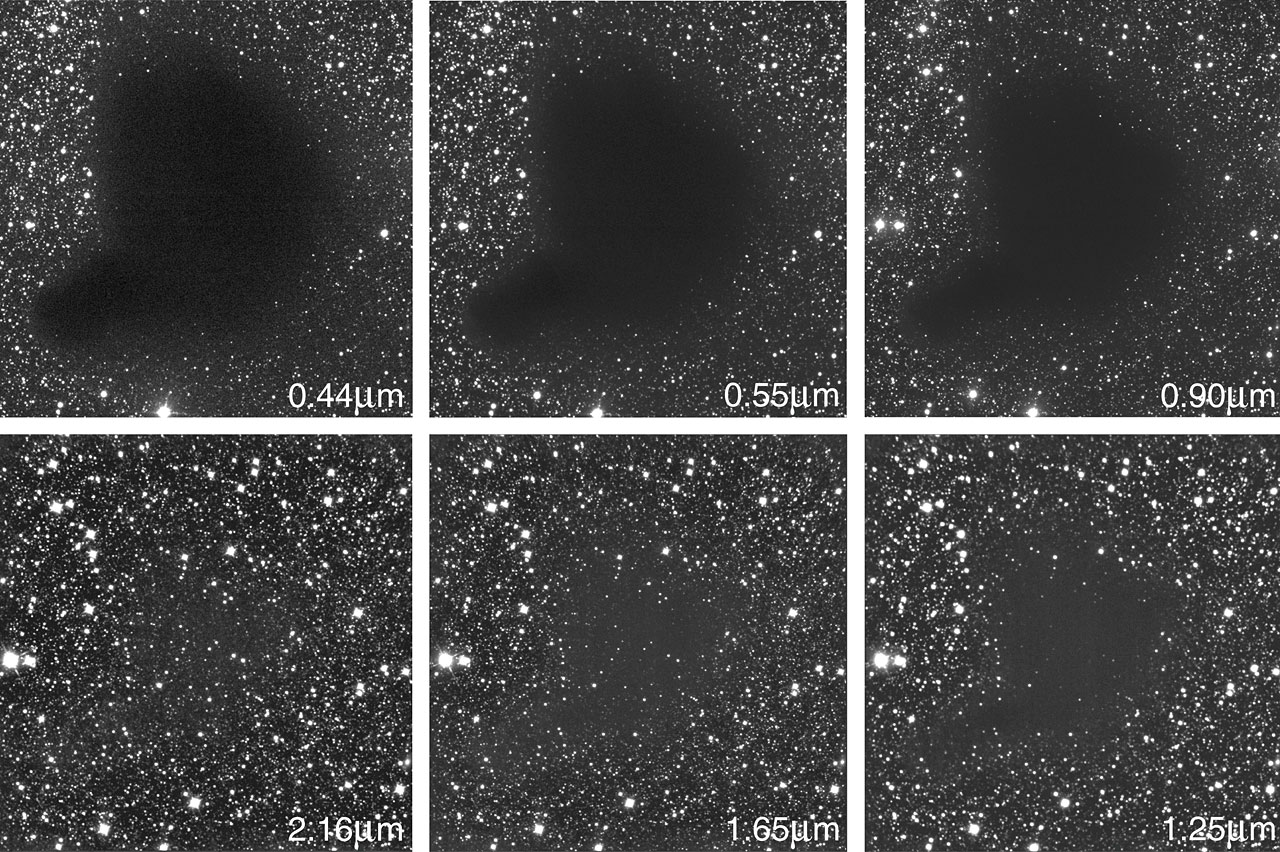
\includegraphics[width=4.5in]{star-formation/figs/eso9934b}
  \caption{Barnard 68, a classic ``Bok globule.'' This turns out to be a stellar nursery, with the young stars embedded in an opaque (at optical wavelengths) shroud. William Herschel was the first astronomer to discover such ``nebulae'' as this one, upon which he exclaimed, ``My god! There's a hole in the sky!''}\label{f.bok}
\end{figure}

Molecular clouds are optically thick to visible and UV photons.
Figure \ref{f.bok} shows images of a molecular cloud at various different wavelengths.
At optical wavelengths, the cloud is clearly opaque, but at longer wavelengths into the IR, the cloud becomes transparent, revealing young stars embedded within.
The cooling of such clouds is thus dominated by emission in the IR where the clouds are transparent.
The main drivers of this cooling are emission by molecules and by dust.
The cooling is sufficiently efficient that the collapse is essentially {\it isothermal}, occurring at roughly constant temperature throughout.
This overcomes the increasing Jeans' mass catastrophe mentioned above, allowing the continued collapse of unstable clouds.

\newthought{Fragmentation} of the molecular clouds occurs as they collapse.
This happens since, for isothermal collapse, the Jeans' mass decreases as $\rho^{-1/2}$ and so smaller overdensities become Jeans unstable and collapse within the overall collapsing cloud. That is, the Jeans {\it length} decreases faster than the overall size of the cloud.
Smaller and smaller fragments collapse faster and faster leading to a hierarchical breakup of the overall cloud and a distribution of so-called {\it clump} masses.
These clumps will become protostars and, eventually, stars proper.
Fragmentation of molecular clouds occurs down to a minimum mass of about 0.01 \Msun.

Collapse clumps eventually become stars, but this process is rather inefficient.
Massive stars form first (because more massive clumps have shorter free-fall times, and well, every other time scale is also short!).
The winds and ultimate explosions of these stars drive gas out of star forming regions.
Roughly, only about 10\% of the original mass of a giant molecular cloud makes it into newborn stars.

\begin{exercisebox}[The minimum mass of stars.]
  In this exercise you will show that the minimum mass of a star collapsing via the Jeans instability is
  \begin{equation}
    M_\mathrm{min} \approx 10^{-2}\ \Msun. \label{e.min-jeans-mass}
  \end{equation}
  As discussed above, in order for a clump to continue collapsing, it must be able to radiate away the liberated gravitational binding energy, at a minimum. In other words,
  \[L_\mathrm{clump} > -\frac{\dif E_\mathrm{grav}}{\dif t}.\]
  The cooling will become inefficient was the clump is sufficiently dense to be optically thick to IR photons, at which point it will radiate like a black body (that's a {\it hint}).
  Finally, since the clump being considered did in fact collapse, you may assume it is of at least the Jeans' mass (Eq. \ref{e.jeans-mass}).
  Given all the above, show that the minimum clump mass that will gravitationally collapse is indeed Eq. (\ref{e.min-jeans-mass}).
\end{exercisebox}

\section{The End of Free-fall and the Birth of a Protostar}

During the free-fall phase, a contracting clump remains transparent to the IR photons that dominate the cooling.
Once the clump becomes sufficiently dense, however, it becomes opaque to the molecular cooling photons and the isothermal contraction turns to adiabatic contraction, at least for the inner core of the clump.
This drives the temperature up ($T\sim\rho^{2/3}$).
Eventually, the high temperatures will dissociate the H$_2$ molecules, robbing the core of its principle coolant, further exacerbating the increase in temperature.
Ultimately, the atomic hydrogen is ionized.
The temperature, and hence pressure, will rise enough to bring the clump into hydrostatic equilibrium, at which point we may consider it a {\it protostar}.

We can estimate the conditions at the end of the free-fall phase by considering the energetics of H$_2$ dissociation and H ionization.
Dissociating a H$_2$ molecule requires an energy $x_\mathrm{H2}=4.5$ eV while the ionization potential is $x_\mathrm{H}=13.6$ eV.\sidenote{Recall, 1 ev = $1.602\times10^{-12}$ erg.}
So, assuming a hydrogen fraction $X=0.7$ and a helium fraction $Y=0.3$, the total energy to dissociate and ionize all the hydrogen in a clump is
\begin{eqnarray*}
  E_\mathrm{dis,ion} &=& \frac{M X}{\mb}(0.5x_\mathrm{H2} + x_\mathrm{H}) \\
  &=& 1.3\times10^{58} \frac{M}{\Msun}\ \mathrm{eV} \approx 2\times10^{46} \frac{M}{\Msun}\ \mathrm{erg}.
\end{eqnarray*}
This energy is provided by released gravitational binding energy due to the collapse
\begin{eqnarray*}
  \Delta
\end{eqnarray*}

\section{The Hayashi Track}\label{s.Hayashi}

For a fully convective star, we can use the fact that the entropy per unit mass is the same at the photosphere as at the center to relate the surface temperature to the mass and radius of the star. Namely,
\begin{equation}\label{e.Teff-adiabat}
\Teff = T_{c}\left(\frac{P_{\mathrm{ph}}}{P_{c}}\right)^{2/5},
\end{equation}
with
\begin{eqnarray}
T_{c} &=& 0.5 \frac{GM\mu \mb}{kR} \label{e.fc-Tc}\\
P_{c} &=& 0.8\frac{GM^{2}}{R^{4}} \label{e.fc-Pc}
\end{eqnarray}
being the central density and pressure of a polytrope of index $n=3/2$, and $P_{\mathrm{ph}}$ being the root of the equation
\begin{equation}\label{e.pph}
 P_{\mathrm{ph}} \approx \frac{GM}{R^{2}}\frac{1}{\kappa_{0}(\mu\mb/k)^{r}P_{\mathrm{ph}}^{r}\Teff^{s-r}}.
\end{equation}
(We could have used the solution for $P(\tau)$ from before, but this approximation is accurate enough to demonstrate our point.)

Now for some crazy fractions: insert equations~(\ref{e.fc-Tc}), (\ref{e.fc-Pc}), and (\ref{e.pph}) into equation~(\ref{e.Teff-adiabat}) and solve for $\Teff$ to find
\begin{equation}\label{e.Teff-MR}
\Teff^{5+3r+2s} = 0.55^{5(1+r)}\kappa_{0}^{-2} \left(\frac{G\mu\mb}{k}\right)^{5+3r}M^{3+r} R^{3r-1}.
\end{equation}
What does this say for Thomson scattering ($\kappa_{0} \approx 0.4$, $r=s=0$)? Inserting these values into eq.~(\ref{e.Teff-MR}) gives
\begin{equation}\label{e.Teff-th}
	\Teff \approx 250\nsp\K \left(\frac{M}{\Msun}\right)^{3/5}\left(\frac{R}{R_{\odot}}\right)^{-1/5},
\end{equation}
a ridiculous value. Let's try it with H$^{-}$ opacity ($\kappa_{0} \approx 2.5\ee{-31}$, $r=1/2$, $s=9$). In this case,
\begin{equation}\label{e.Teff-H-}
 \Teff \approx 2200\nsp\K \left(\frac{M}{\Msun}\right)^{1/7}\left(\frac{R}{\Rsun}\right)^{1/49}.
\end{equation}
Note the extremely weak dependence on $R$.  This is a consequence that $R$ is very sensitive to the entropy at the photosphere.  Writing $L = 4\pi R^{2}\ssb \Teff^{4}$, we can solve for $R$ and insert it into equation~(\ref{e.Teff-H-}) to get the effective temperature in terms of mass and luminosity,
\begin{equation}\label{e.Hayashi}
 \Teff \approx 2300\nsp\K \left(\frac{M}{\Msun}\right)^{7/51}\left(\frac{L}{L_{\odot}}\right)^{1/102}.
\end{equation}
This is a crude estimate, so don't take these numbers too seriously. What this exercise illustrates, however, is that the effective temperature for fully convective, low-mass stars is essentially independent of luminosity.  On an HR diagram, these stars follow a vertical track, known as the \emph{Hayashi track}, as they contract to the main sequence.

\begin{figure}[htbp]
  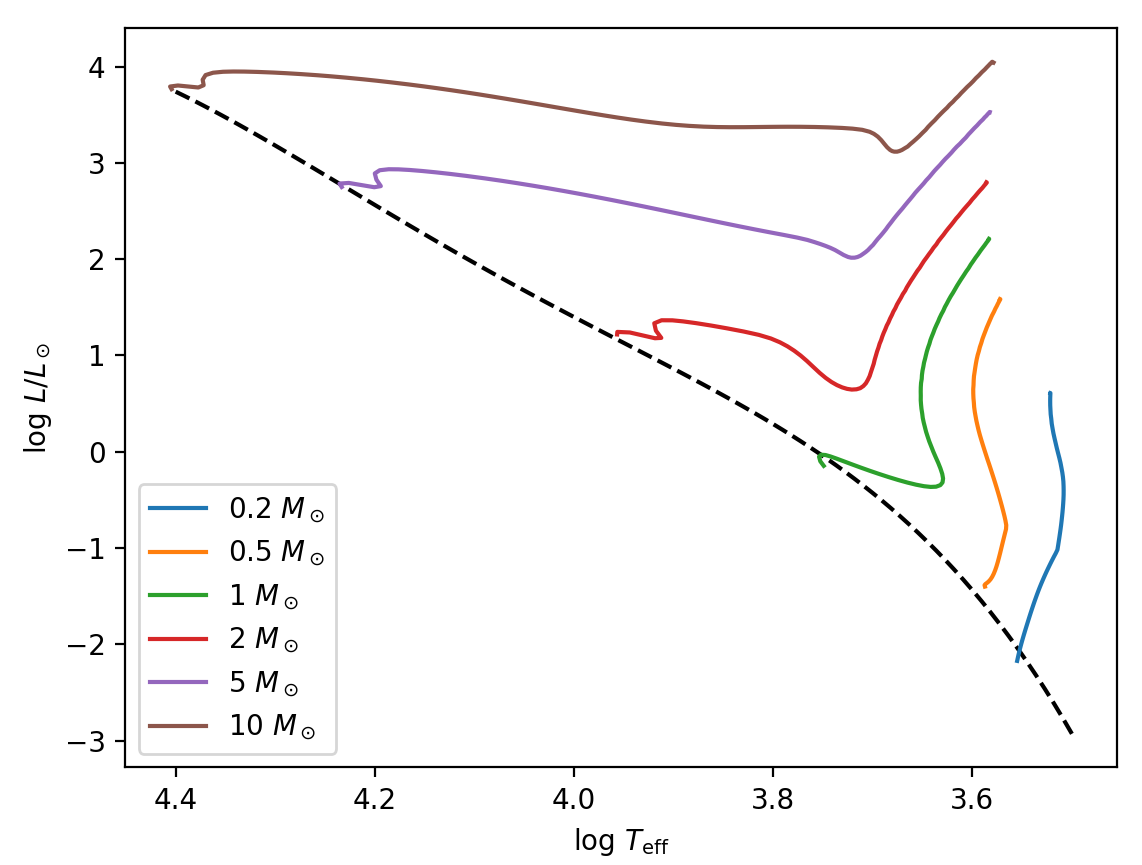
\includegraphics[width=4in]{star-formation/figs/hayashi}
  \caption{Pre-main sequence tracks for stars of several different masses. The main sequence is represented by the dashed line.
  The Hayashi tracks are the roughly vertical, constant temperature lines on the right while the radiative, protostar phases are the horizontal, constant luminosity lines.}\label{f.hayashi}
\end{figure}

The HR diagram in Figure \ref{f.hayashi} shows the pre-main sequence evolution for stars of various masses.
The tracks begin in the upper right of the diagram.
The Hayashi phase is the roughly vertical portion.


\section{Formation of a radiative core}

For low-mass stars, the opacity in the core has a Kramers'-like form, $\kappa \propto \rho T^{-7/2}$. From our scalings, we see that $\kappa \propto M^{-5/2} R^{1/2}$.  As a result, as the star contracts, the central opacity decreases.  If it decreases enough, then photons can carry the flux and a radiative core will develop.

To find out when a radiative core forms, let's start with our equation for the flux,
\[ F(r) = -\frac{1}{3}\frac{c}{\rho\kappa}\frac{\dif aT^{4}}{\dif r}, \]
and use hydrostatic balance to rewrite this as
\[ L(r) = 4\pi r^{2}F(r) = \frac{16\pi}{3}  \frac{acT^{4}}{\kappa} \frac{Gm(r)}{P} \frac{\dif \ln T}{\dif \ln P}. \]
Now imagine we consider a tiny amount of matter $\delta m$ about the center of the star.  The luminosity coming out of this sphere is $\delta L(r)$,  and since in a convectively stable atmosphere $\dif\ln T/\dif\ln P < (\Gamma_{2}-1)/\Gamma_{2}$, the maximum amount of energy that can be generated in the sphere $\delta m$ and transported away in the absence of convection is
\begin{equation}\label{e.max_deltaL}
  \frac{\delta L(r)}{\delta m} < \frac{16\pi}{3} \frac{Gac}{\kappa} \frac{T_{c}^{4}}{P_{c}}  \frac{\Gamma_{2}-1}{\Gamma_{2}}.
\end{equation}
Flashback! Do you remember doing problem \ref{p.lagrange-heat} of chapter \ref{ch.stellar-structure-eqn}? This gave us an expression, eq.~(\ref{e.lagrange-heat-alt2}), for $\partial L/\partial m$, which we can equate with the LHS of equation~(\ref{e.max_deltaL}):
\[
 q - \frac{P_{c}}{\rho_{c}(\Gamma_{3}-1)}\frac{\Dif }{\Dif t}\ln\left(\frac{P_{c}}{\rho_{c}^{\Gamma_{1}}}\right) <
 	\frac{16\pi}{3} \frac{Gac}{\kappa} \frac{T_{c}^{4}}{P_{c}}  \frac{\Gamma_{2}-1}{\Gamma_{2}}.
\]
Let's do the time warp again: in problem \ref{p.radius-entropy} of chapter \ref{ch.polytropes}, you showed that $P/\rho^{\Gamma_{1}} \propto R$ for an ideal gas (i.e., the polytropic constant $K$); making this substitution in the derivative gives the condition for the formation of a radiative core,
\begin{equation}\label{e.formation-radiative-core}
q - \frac{\NA\kB T_{c}}{\mu(\Gamma_{3}-1)} \frac{\Dif \ln R}{\Dif t} < \frac{16\pi}{3} \frac{Gac}{\kappa} \frac{T_{c}^{4}}{P_{c}}  \frac{\Gamma_{2}-1}{\Gamma_{2}}.
\end{equation}
Stars with $M \gtrsim 0.3 \Msun$ form a radiative core while contracting to the main-sequence; in contrast, lower-mass stars remain fully convective throughout their main-sequence lives.

\begin{exercisebox}[Contraction of a low-mass pre-main-sequence star]
We showed that low-mass pre-main-sequence stars (including brown dwarfs) are fully convective and have nearly constant effective temperatures.  Use these facts to model their pre-main sequence contraction.  Assume $T_{\mathrm{eff}} = \mathrm{const.}$ so that the luminosity is $L = 4\pi R^{2} \sigma_{\mathrm{SB}} T_{\mathrm{eff}}^{4}$.

\begin{enumerate}
\item Use the appropriate polytropic relation for the energy of the protostar and assume that the luminosity is entirely powered by contraction, i.e., the star is not yet approaching the main-sequence. Derive an equation for $R(t)$. What is the characteristic timescale for a low-mass star to contract? Scale your answer to $T_{\mathrm{eff}} = 3000\nsp\K$ and $M = 0.1\nsp\Msun$ (i.e., get an analytical solution in terms of the variables $\tilde{T} = [\Teff/3000\nsp\K]$ and $\tilde{M} = [M/0.1\nsp\Msun]$).

\item Compare your findings with more elaborate calculations.  You will find a review in \href{http://arxiv.org/abs/astro-ph/0006383}{``Theory of Low-Mass Stars and Substellar Objects,''} G. Chabrier and I. Baraffe, Ann.\ Rev.\ Astron.\ Astrophys.\ \textbf{38:} 337 (2000).
%\item Using appropriate expressions for the central density and temperature, calculate the time required for a star just below the hydrogen burning limit (about $0.07\nsp\Msun$) to contract to a radius such that $\eF(\rho_{c}) = \kB T_{c}$, where $\eF$ is the Fermi energy, and compare with the evolutionary tracks in Chabrier \& Baraffe.
\end{enumerate}
\end{exercisebox}

\section{The Initial Mass Function}
\newcommand{\tms}{\ensuremath{\tau_{\mathrm{MS}}}}
\newcommand{\tauG}{\ensuremath{\tau_{\mathrm{G}}}}
\newcommand{\AIa}{\ensuremath{A_{\mathrm{Ia}}}}

As originally formulated\cite{Salpeter1955The-Luminosity-}, the initial mass funciton (IMF) is the number of stars, per unit volume, that have formed per logarithmic (base 10) mass interval:
\begin{equation}\label{e.IMF}
\xi(\lg m) \equiv \frac{\dif(N_{\star}/V)}{\dif\lg m}.
\end{equation}
Here $m \equiv M/\Msun$.
The IMF is derived from an observed \emph{luminosity function}---the amount of starlight in a given waveband emitted per unit mass---and stellar models.  As might be expected, this function is not well-constrained, but it is roughly a power law for $m > 1.0$, and at lower masses it flattens out. One such formulation\cite{Chabrier2003Galactic-Stella} for the solar neighborhood is
\begin{equation}\label{e.IMF-chabrier}
\xi(\lg m) = \left\{\begin{array}{lr}A_0\exp\left[-\frac{(\lg m - \lg m_c)^2}{2\sigma^2}\right], & m < 1.0 \\A_1 m^b & m > 1.0\end{array}\right. .
\end{equation}
Here $A_{0} = 0.158$, $A_{1} = 4.43\ee{-2}$, $m_{c} = 0.079$, $\sigma = 0.69$, and $b = -1.3\pm 0.3$.  The coefficients $A_{0}$, $A_{1}$ are in $\lg\Msun^{-1}\usp\parsec^{-3}$.

\begin{exercisebox}[Fraction of stars forming core-collapse supernovae]
 For the IMF given in eq.~(\ref{e.IMF-chabrier}), what fraction of the stars formed with $m > 1.0$ will end their lives as core-collapse supernovae, if the mass threshold for forming a core-collapse SNe is $8.0\nsp\Msun$?  What is the fraction if the mass threshold is $12.0\nsp\Msun$?
\end{exercisebox}

\begin{figure}[htbp]\caption{title}
  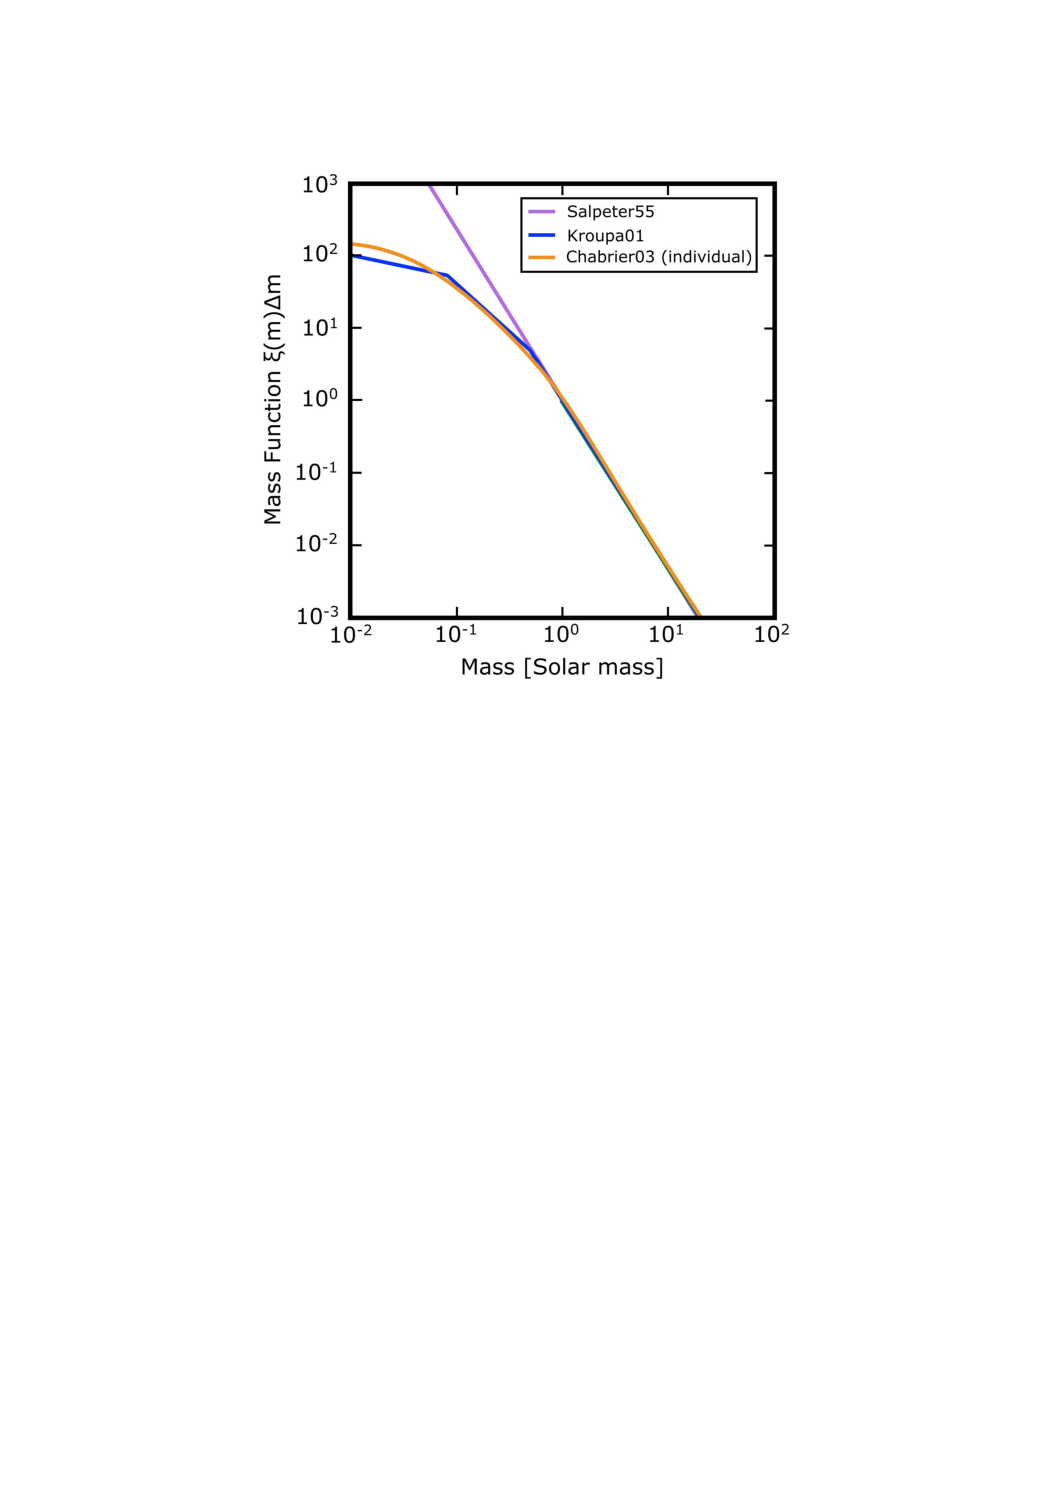
\includegraphics[width=3in]{star-formation/figs/imf}
\end{figure}
The main-sequence lifetime is a rapidly decreasing function of mass: for $m > 1.0$, it goes roughly like $\tms \approx 10.0\nsp\Giga\yr\nsp m^{-2.5}$. For stars with lifetimes comparable to or longer than the age of the galactic disc $\tauG$, all stars that were ever formed are still on the main sequence, so that the IMF is identical to  the \emph{present day mass function} (PDMF) $\phi$.  For more massive stars, however, we only see those that were formed a time $\tms(m)$ ago.

Let's define a birthrate $B(t)$ as the number of stars per unit volume formed per interval of time.  If we make the \emph{ansatz} that the IMF doesn't depend on time, then we can define a creation function,
\begin{equation}\label{e.creation-fcn}
C(\lg m,t) \equiv \xi(\lg m)\frac{B(t)}{\int_{0}^{\tauG} B(t)\,\dif t}.
\end{equation}
Here the birthrate is normalized to the total number of stars formed over the age of the galactic disk. The present-day mass function is then
\[
	\phi(\lg m) = \int_{\max(0,\tauG-\tms)}^{\tauG} C(\lg m,t) \dif t.
\]
For a constant birthrate over the age of the disk, the integral is trivial and
\[
	\phi(\lg m) = \left\{\begin{array}{lr}\xi(\lg m)\frac{\tms(m)}{\tauG} & \tms < \tauG \\
		\xi(\lg m) & \tms > \tauG\end{array}\right.
\]
As the galaxy ages, the stellar population becomes increasingly dominated by long-lived, low-mass stars.
Empirically, the Milky Way birthrate has in fact been more or less constant (deviations less than a factor of 2) over the life of the galactic disk.  The timescale for converting the present supply of gas into stars is $\sim (1\textrm{--}5)\Giga\yr$.

For an IMF, we can define, for each generation of stars, a \emph{lock-up fraction}, which is the amount of gas that is not eventually returned to the interstellar medium. Clearly this will include all stars with $\tms(m) > \tauG$, as well as the remnant mass, $m_{\mathrm{rem}}(m)$, of the remaining stars.  For stars with mass $< 8\nsp\Msun$, the mass of the white dwarf as a function of the progenitor's mass is fairly well known; more massive stars leave behind either a neutron star, for which observed masses (in binaries!) are 1--2\nsp\Msun; for black holes the remnant mass is more uncertain.

\begin{exercisebox}[Number of stars formed per solar mass of gas]
Suppose the IMF is simply a power-law, $\xi(\lg m) \propto m^{-1.3}$, for $0.1 < m < 120$. On average, how many stars are formed out of one solar mass of gas?
\end{exercisebox}

\section{Application: The delay time of type Ia supernovae}\label{s.delay-time}

Type Ia supernovae are observed in elliptical galaxies, which typically have an old stellar population and no ongoing star formation.  There must be a substantial delay, then, between the time the progenitor was born and the supernovae.  To see how this works, let's define a \emph{delay time distribution} $\mathcal{D}(\tau)$ and a \emph{realization probability} $\AIa(t)$. These are defined as follows: if $N_{\star}(t)$ is the total number of stars formed at time $t$, then define $N_{\star}(t)\AIa(t)$ as the total number of SNe Ia that will ever result from this generation of stars. The SNe Ia rate at the current time, $t =\tauG$, is then
\begin{equation}\label{e.Ia-rate}
\Gamma_{\mathrm{Ia}}(t=\tauG) = \int_{\tau_{\min}}^{\min(\tauG,\tau_{\max})}\,\int_{\lg m_{\min}}^{\lg m_{\max}}\,C(\lg m,t-\tau) \AIa(t-\tau) \mathcal{D}(\tau)\,\dif\lg m\,\dif\tau.
\end{equation}
In this definition, the delay time distribution is normalized to unity.

As an example, suppose all the stars are born in a burst of star formation at $t=0$, so that $B(t) = \delta(t)$, then the SNe Ia rate at late times is
\[
\Gamma_{\mathrm{Ia}}(t=\tauG) = \int_{\tau_{\min}}^{\min(\tauG,\tau_{\max})}\,N_{\star}\delta(t-\tau) \AIa(t-\tau) \mathcal{D}(\tau)\,\dif\tau = N_{\star}\AIa\mathcal{D}(t).
\]
Notice that if $\mathcal{D}(t)$ is a very broad function of time, then the SNe Ia rate is proportional, for this case of a rapid burst of star formation at early times, to the total number of stars in the galaxy.


\begin{exercisebox}[The Type Ia SNe rate]
Consider the SNe Ia rate, eq.~(\ref{e.Ia-rate}), following a burst of star formation, $B(t) = \delta(t)$, but now suppose that the delay time for each mass is just the main-sequence lifetime, and that $\AIa$ is independent of mass. That is, for stars with mass $m =  M/\Msun< 8$, we assume that some fraction $\AIa$ will become SNe Ia, and that the time for a particular mass star to evolve to explosion is just its main-sequence lifetime $\tau(m) = \tms(m)$. Show that, for $\xi(\lg m) \propto m^{-1.3}$ and $\tms = 10.0\nsp\Giga\yr \nsp m^{-2.5}$, the Ia rate is $\Gamma_{\mathrm{Ia}} \propto t^{-0.5}$, for $t > \tms(m=8)$.
\end{exercisebox}
